\begin{frame}{Conclusions and plans}

    \begin{tikzpicture}[overlay, remember picture]
        \node at (current page.center) {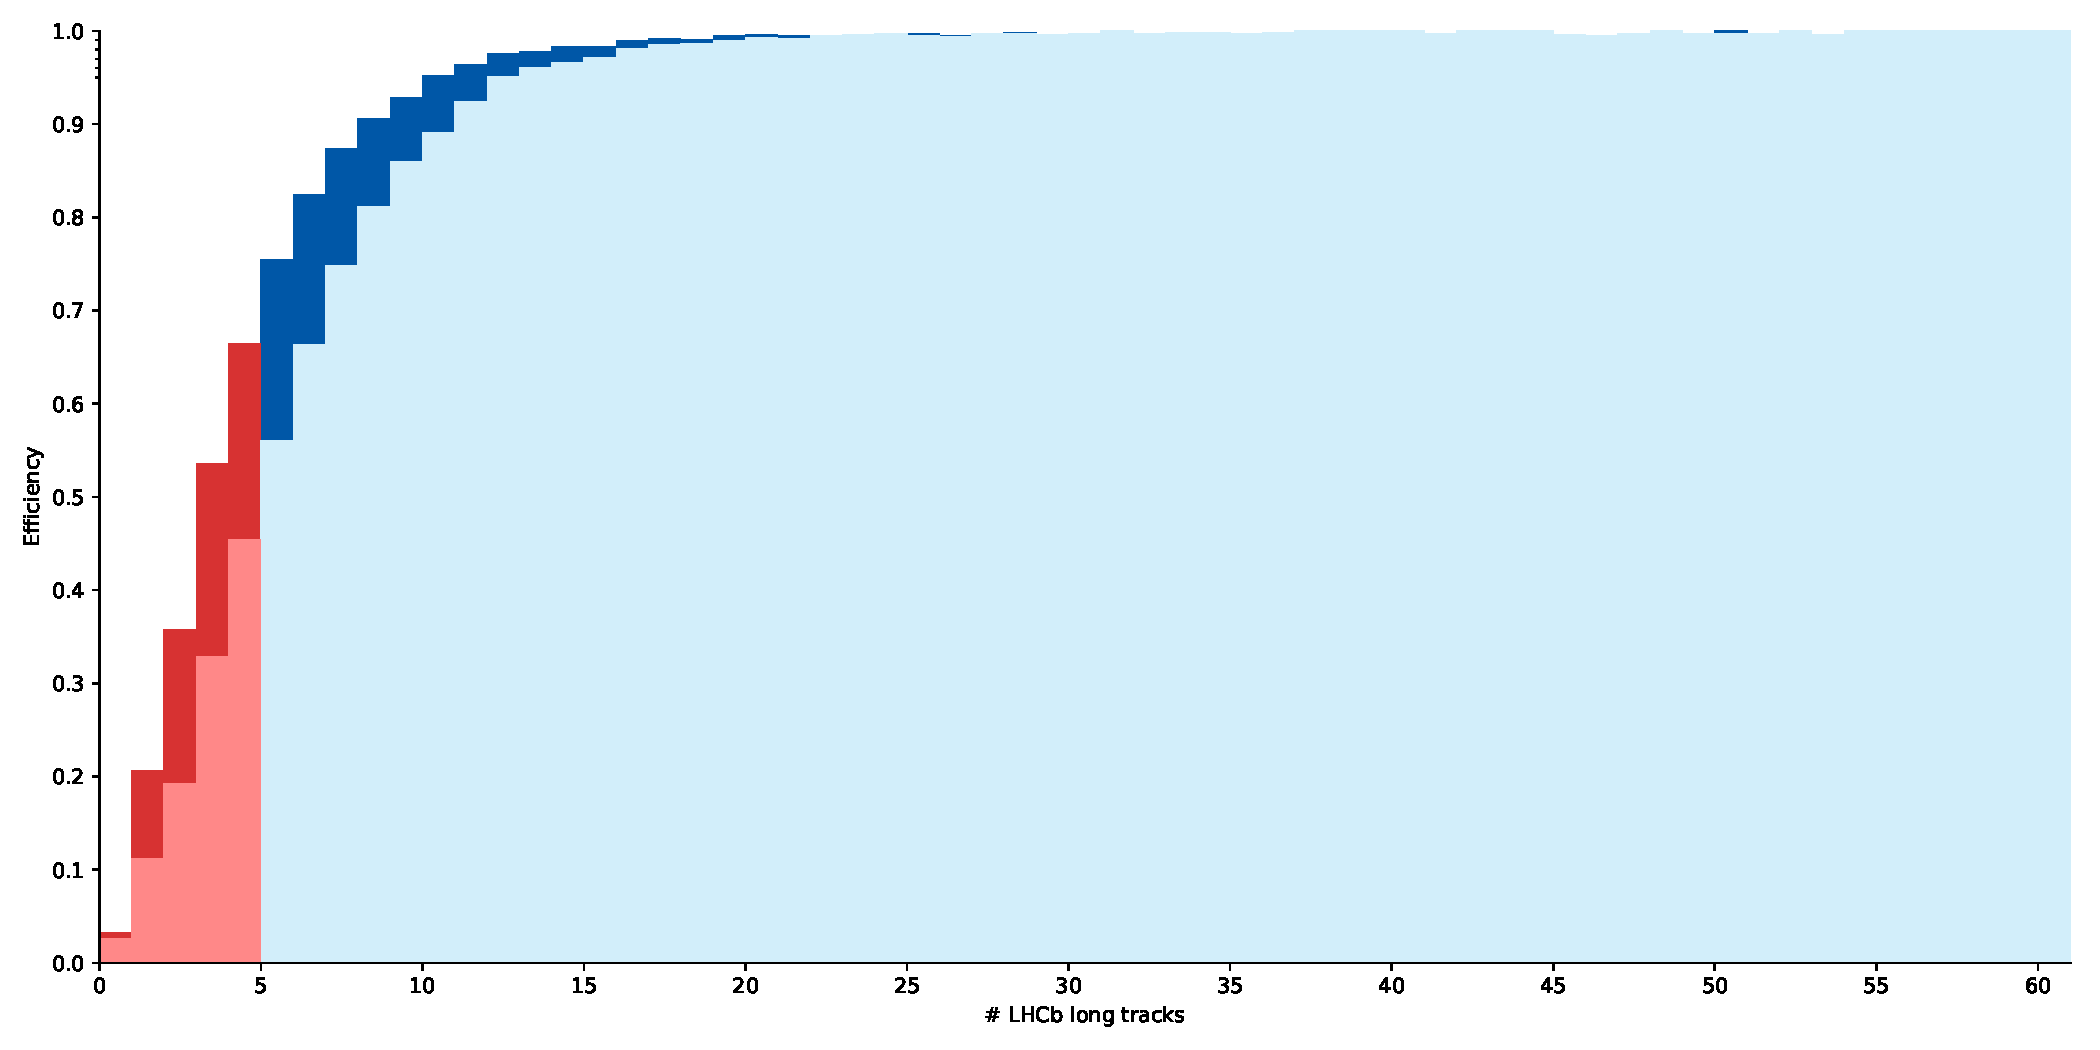
\includegraphics[width=12cm]{images/effntracks_bg.pdf}};
    \end{tikzpicture}
\begin{columns}
\column{.25\textwidth}
\column{.65\textwidth}
\setstretch{0.92}
\vskip -1.75em
    \begin{itemize}
    \setlength\itemsep{0.25em}
        \item [\textcolor{yellow}{\textbullet}] \color{yellow} 
          Proof-of-Principle established:
          \color{lhcbLightBlue}
          a hybrid ML algorithm using a 1-dimensional KDE processed by a 5-layer CNN finds primary vertices with efficiencies and false positive rates similar to traditional algorithms.
        \item [\textcolor{yellow}{\textbullet}] \color{yellow} Efficiency is tunable; \color{lhcbLightBlue} increasing the efficiency also increases the false positive rate.
        \item [\textcolor{yellow}{\textbullet}] \color{yellow} Adding information
        should improve performance.
        \color{lhcbLightBlue}
        \begin{itemize}
            \item [\textcolor{lhcbLightBlue}
            {\textbullet} \color{lhcbLightBlue}] \color{lhcbLightBlue}
            can add KDE (x,y) information to algorithm
            \item [\color{lhcbLightBlue}{\textbullet} \color{lhcbLightBlue}]
            \color{lhcbLightBlue} can associate tracks to PV candidates, then iterate.
        \end{itemize}
        \item [\textcolor{yellow}{\textbullet}] \color{yellow} Next steps:
        \color{lhcbLightBlue}
        train with full LHCb MC and deploy inference engine in LHCb Hlt1 framework.
        \item [\textcolor{yellow}{\textbullet}] \color{yellow} Beyond LHCb
        \begin{itemize}
            \item [\color{lhcbLightBlue} {\textbullet}] \color{lhcbLightBlue}
            approach might work for ATLAS and CMS;
            \item [\color{lhcbLightBlue} {\textbullet}] \color{lhcbLightBlue} algorithm is an interesting ML laboratory.
        \end{itemize}
    \end{itemize}
\column{.1\textwidth}
\end{columns}
\end{frame}
